% siminos/atlas/intro.tex  pdflatex atlas
% $Author$ $Date$

\begin{quotation}
    \ifdraft\color{blue}
The ``lead paragraph'' is formatted as a single paragraph before the first
section heading. Numbered references are allowed.
        \PC{
    The first paragraph of the article should be a Lead Paragraph and
    will be highlighted in the journal in boldface type. This paragraph,
    which essentially advertises the main points of the article, must
    describe in terms accessible to the nonspecialist reader the context
    and significance of the research problem studied and the importance
    of the results. The Editors will pay special attention to the clarity
    and accessibility of this paragraph, and in many cases may rewrite it
        }
    \color{black}\fi
\end{quotation}

    \PC{2012-01-03 experiment with
    \ensuremath{\hat{\ssp}}, \ensuremath{\bar{\ssp}} or \ensuremath{\tilde{\ssp}}
    as the \reducedsp\ coordinate.
    }

\section{Introduction}
\label{s:intro}
% former siminos/atlas/intro.tex

    \ifdraft\color{blue}
    \PC{
{\bf 2012-03-12 Predrag} A putative outline of the paper is in
\refsect{chap:outline}.
    }
Goal: chart the regions of \statesp\ explored by chaotic dynamics,
a curved manifold embedded in a high-dimensional \statesp..

Key notion: recurrence.
To quantify `near' need the notion of distance, or 'norm'.

Problem: evolution in time decomposes \statesp\ into spaghetti of time
orbits or trajectories. Symmetries stratify it into layers of an onion.
Need to pick a single point for each trajectory and each group orbit.

(template)

Cover the curved manifold by the shortest-distance sections (for time
recurrence) and \slice s (for continuous shifts). In the limit of longer
and longer cycles this leads to the usual curved manifold geometry,
measured locally by Euclidean distances.
    \color{black}\fi

Recent insights in the theory of higher-dimensional chaotic dynamical systems
necessitate reexamination of two of the basic tools of the theory of
dynamical systems, Poincar\'e sections and symmetry reduction.

Over the last decade, researchers have gained new insights into the theory of higher-dimensional chaotic dynamical systems. These developments offer a promising dynamical framework to with which to study turbulence. In this picture, turbulence is viewed as a walk through a forest of exact solutions of the governing equations with each solution shaping the local \statesp\ dynamics. 

%Making full use of these ideas necessitates reexamination of two of the basic tools of the theory of dynamical systems, Poincar\'e sections and symmetry reduction.

Taking this approach, the dynamics of moderate \Reynolds\ turbulent flows are
visualized in the $\infty$-dimensional \stateDsp\  using \eqv\ solutions
of the \NSe\ to construct dynamically invariant, intrinsic, and
representation independent coordinate frames \rf{GHCW07}. Visualizing of turbulent flows in these frames inform a new way of thinking about the role {\recurrStr s}
that play in shaping turbulence: The observed {\cohStr s} are the physical images of the flow's least unstable invariant solutions, with chaotic dynamics arising from a sequence of transitions between these states, and the intrinsic low-dimensionality of turbulence resulting from the low number of unstable eigendirections of these states.
Unstable \po s are of particular importance, as they provide the skeleton underpinning the chaotic dynamics\rf{DasBuch}: the geometry of the \statesp\ flow
near onset of turbulence is shaped by the chaotic saddle, a set of unstable solutions and their heteroclinic connections.

The importance of a given invariant solution is made precise by periodic
orbit theory which assigns a deterministic weight with which the solution
contributes to any dynamical average over the chaotic component of the flow
\rf{DasBuch}. Consideration of continuous symmetries extends this
theory to sums over \emph{relative} periodic orbits\rf{Cvi07}, time-dependent solutions which recur periodically in co-moving frames translating along and/or rotating about the axes of symmetry with different translational and rotational velocities for each solution.

%%%%%%%%%%%%%%%%%%%%%%%%%%%%%%%%%%%%%%%%%%%%%%%%%
% 2011-10-23 Predrag: replace this Ashley' simulation
%            continuous.tex overheads, and ChaosBook
% TEMPORARY: from siminos/rpo_ks/arxiv-v2/figs, \refref{cont:SCD07})
%
\begin{figure}
\centering
(a)%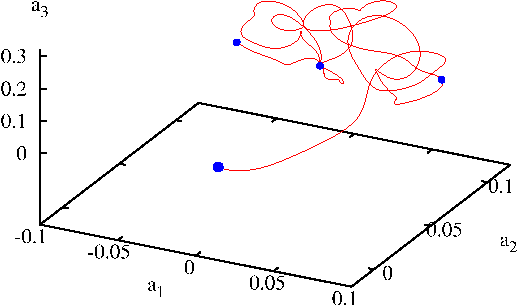
\includegraphics[width=0.45\textwidth,clip=true]{2841GO3a}
~~(b)%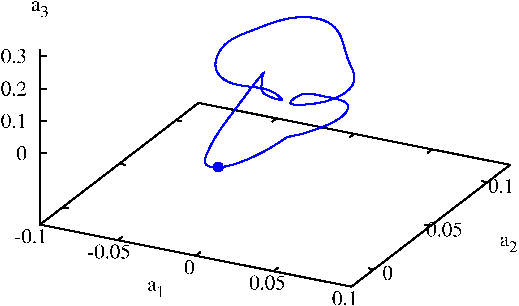
\includegraphics[width=0.45\textwidth,clip=true]{2841GO3b}
  \caption{\label{f:MeanVelocityFrame}
Symmetry reduction $\pS \to \pSRed$ replaces each
(a)
full \statesp\ trajectory $\ssp(\zeit)$ by
(b)
a simpler \reducedsp\ trajectory $\sspRed(\zeit)$, with continuous group
induced drifts quotiented out. Here this is illustrated by the pipe flow \rpo\
$\RPO{36.92}$
(a) %(red)
traced in the full {\statesp} for two $\period{}=36.92$ periods, in the
frame moving with the constant mean axial flow speed $U$;
(b) %(blue)
restricted to the symmetry-\reducedsp. Both are projected onto the
$3$\dmn\ frame \refeq{FrenetFrame1}. In the full \statesp\ a \rpo\ traces
out quasi-periodically a highly contorted 2-torus; in the \reducedsp\ it
closes a \po\ in one period $\period{}$.
            }
\end{figure}
%%%%%%%%%%%%%%%%%%%%%%%%%%%%%%%%%%%%%%%%%%%%%%%%%%

Visualizing a single `relative' orbit in its co-moving frame is useful if we are concerned with that individual solution. Unfortunately, it is useless if we are concerned with studying collections of these orbits since different orbits do not share the same co-moving frame.

\PC{
{\bf 2012-03-28 Daniel} I think that at this point the writing kind of abruptly jumps from goody-goody intro for the everyman to technical without sufficient warning. Need to segway into the group theory stuff}

This problem is here resolved by the {\mslices}\rf{rowley_reconstruction_2000,BeTh04,SiCvi10,FrCv11}, in
which the group orbit of any full-flow structure is represented by a
single point (see \reffig{fig:BeThTraj}), the group orbit's intersection
with a fixed hypersurface, or the \emph{`\slice'}. A
\slice\ fixes only the symmetry group phases: a continuous time full space
orbit is reduced to a continuous time orbit in the symmetry-\reducedsp,
as in \reffig{f:MeanVelocityFrame}.

Our goals here are two-fold:
(i) First, we review the method of Poincar\'e sections,
    in order to motivate the need for for symmetry reduction, explain 
    what it is, and how with it the geometry of \statesp\ dynamics is revealed;
(ii) Next, we demonstrate that this tool enables us to commence a systematic
exploration of the hierarchy of dynamically important invariant solutions
of flows with continuous symmetries. The $\infty$-dimensional \stateDsp\
representation\rf{GHCW07} of PDEs, such as \reffig{f:MeanVelocityFrame},
enables us to track the unstable manifolds of invariant
solutions, the heteroclinic connections between them\rf{GHCV08}, and
{provides us with} new insights into the nonlinear \statesp\ geometry and
dynamics of moderate \Reynolds\ wall-bounded flows.

We review  ??? flows, their visualization, and their symmetries in
\refsect{s:review}. The {\mslices}  is described in \refsect{s:slice},
and the computation of invariant solutions and their stability
eigenvalues and eigenvectors in \refsects {sect:TimeOrb}{s:algorithm}.
The main advances reported in this paper are the symmetry \reducedsp\
visualization and [...], (\refsect{s:rpos}). Outstanding challenges are
discussed in \refsect{s:concl}.
